\documentclass[9pt]{article}

% if you need to pass options to natbib, use, e.g.:
%     \PassOptionsToPackage{numbers, compress}{natbib}
% before loading neurips_2020

% ready for submission
% \usepackage{neurips_2020}

% to compile a preprint version, e.g., for submission to arXiv, add add the
% [preprint] option:
\usepackage[preprint]{neurips_2020}

% to compile a camera-ready version, add the [final] option, e.g.:
%     \usepackage[final]{neurips_2020}

% to avoid loading the natbib package, add option nonatbib:
%     \usepackage[nonatbib]{neurips_2020}

\usepackage[utf8]{inputenc} % allow utf-8 input
\usepackage[T1]{fontenc}    % use 8-bit T1 fonts
\usepackage{hyperref}       % hyperlinks
\usepackage{url}            % simple URL typesetting
\usepackage{booktabs}       % professional-quality tables
\usepackage{amsfonts}       % blackboard math symbols
\usepackage{nicefrac}       % compact symbols for 1/2, etc.
\usepackage{microtype}      % microtypography

\usepackage{todonotes}

\usepackage{bm}
\usepackage{amsmath}
\usepackage{graphicx}

% figures
\graphicspath{{./../plots/}}
\usepackage{tikz}
\usetikzlibrary{arrows,backgrounds,positioning,intersections}
\usepackage{pgfplots}
\pgfplotsset{compat=newest}
\usepgfplotslibrary{groupplots}
\usepgfplotslibrary{polar}
\usepgfplotslibrary{smithchart}
\usepgfplotslibrary{statistics}
\usepgfplotslibrary{dateplot}


\newcommand{\real}{\text{Re}}
\newcommand{\imag}{\text{Im}}
\newcommand{\wre}{w_{r}}
\newcommand{\wim}{w_{i}}
\newcommand{\Wre}{\bm W_{r}}
\newcommand{\Wim}{\bm W_{i}}

% tables
\usepackage{booktabs}
\renewcommand{\arraystretch}{1.2}

\title{Neural Power Unit \\-- A Bayesian Approach To Neural Arithmetic}
\author{
  Niklas Heim,
  V\'aclav \v Sm\'idl,
  Tom\'a\v s Pevn\'y \\
  Artificial Intelligence Center\\
  Czech Technical University\\
  Prague, CZ 120 00\\
  \texttt{\{niklas.heim, vasek.smidl, tomas.pevny\}@aic.fel.cvut.cz}\\
}

\begin{document}

\maketitle

\begin{abstract}
  Common Neural Networks can approximate simple arithmetic operations, but fail
  to generalize beyond the range of numbers that were seen during training. A
  new class of units called \emph{Neural Arithmetic Units} aim to overcome this
  difficulty, but are limited either to operate on positive numbers (NALU by
  \citet{trask_neural_2018}), or can only represent simple addition and
  multiplication (NAU \& NMU by \citet{madsen_neural_2020}).  We introduce a
  Neural Arithmetic Unit that operates on the full domain of real numbers and
  is capable of learning arbitrary power functions called \emph{Neural Power
  Unit} (NPU). The NPU enables not only the learning simple arithmetic
  operations, but is also capable of learning e.g. Taylor expansions with very
  few parameters, which makes the NPU highly explainable.
  \footnote{Implementation of neural arithmetic units:
  \url{https://github.com/nmheim/NeuralArithmetic.jl}}.
\end{abstract}


\section{Introduction}%
\label{sec:introduction}

Numbers and simple algebra are essential not only to human intelligence but
also to the survival of many other
species~\citep{dehaene_number_2011,gallistel_finding_2018}.  This can be taken
as a hint that arithmetic is an important ingredient to a successful,
intelligent agent.  State of the art neural networks are capable of learning
simple arithmetic, but they fail to extrapolate beyond the ranges seen during
training~\citep{suzgun_evaluating_2018,lake_generalization_2018}.  The
inability to generalize to unseen inputs is a fundamental problem that hints at
a lack of \emph{understanding} of the given task. The model merely memorizes
the seen inputs and fails to abstract the true learning task.  The failure of
numerical extrapolation on simple arithmetic tasks has been shown
by~\cite{trask_neural_2018}, who also introduce a new class of \emph{Neural
Arithmetic Units} that show good extrapolation performance on some arithmetic
tasks.

The \emph{Neural Arithmetic Logic Unit} (NALU) can learn addition,
subtraction, multiplication, and division with two severe limitations: the
inputs that the NALU is trained with have to be positive, and should be
significantly larger than zero, otherwise the layer will not converge to
a correct solution.

\cite{madsen_neural_2020} introduce two new arithmetic layers, the \emph{Neural
Addition Unit} (NAU) and the \emph{Neural Multiplication Unit} (NMU).
Stacked, they can learn addition, subtraction, and multiplication and they converge
for any input range. However, the NMU cannot learn division.

Including Neural Arithmetic Units in common neural networks, apart from the
potential increase in extrapolation capabilities, has additional advantages.
They promise to reduce the amount of parameters that are needed for a given
task, can drastically improve the explainability of our models (more on the
explainability of the NPU in Sec.~\ref{sec:neural_power_unit}).  Additionally,
the field of Scientific Machine Learning, which, in part, is concerned with
learning differential equations~\citep{rackauckas_universal_2020} could benefit
from the inductive bias neural arithmetic.


\subsection*{Our Contribution}%
\label{sub:our_contribution}

We introduce a new arithmetic layer called the \emph{Neural Power Unit} (NPU)
which is capable of learning addition, subtraction, and arbitrary power
functions, which includes multiplication and division.
Our approach is inspired by the NALU, but overcomes its limitations to
non-small positive numbers by leveraging the complex plane.

\section{Related Work}%
\label{sec:related_work}

\subsection{Neural Arithmetic Logic Unit}%
\label{sub:neural_arithmetic_logic_unit}

\citet{trask_neural_2018} have demonstrated how severe the extrapolation
problem is even for the simplest arithmetic operations, such as summing or
multiplying two numbers.  In order to increase the power of abstraction of NNs
they propose a \emph{Neural Arithmetic Logic Unit} (NALU) which is capable of
learning arithmetic addition, subtraction, multiplication, and division
$\{+,-,\times,\div\}$ with stunning extrapolation accuracy.  However, the NALU
comes with the severe limitation not being able to handle negative inputs due
to the logarithm in the multiplication part of the NALU:

\begin{align}
  \label{eq:nalu_add}
  \text{Addition: }       & \bm a = \bm W \bm x
                          & \bm W& = \tanh(\hat{\bm W}) \odot \sigma(\hat{\bm M}) \\
  \label{eq:nalu_mult}
  \text{Multiplication: } & \bm m = \exp \bm W(\log(|\bm x|+\epsilon)) & &\\
  \text{Output: }         & \bm y = \bm a \odot \bm g + \bm m \odot (1-\bm g) 
                          & \bm g& = \sigma(\bm G\bm x)
\end{align}
Additionally the NALU has severe convergence problems for small inputs due to
a non-smooth loss surface close to zero, as shown by \cite{madsen_neural_2020}.

\todo{should this be here already?}
With the simple exemplary task of learning a function $f:\mathbb R^2 \rightarrow \mathbb R^2$
\begin{equation}
  \label{eq:xx_xdivy}
  f(\bm x) = f(x,y) = [xy,x/y] = \bm t
\end{equation}
we can demonstrate the strengths and weaknesses of the NALU.  The NALU only
learns successfully if it is trained on positive numbers, so we train with
samples from $\bm x \in \mathcal U^2(0.1,2)$ and plot the error $\epsilon =
|\bm t - \hat{\bm t}|^2$ in Fig.~\ref{fig:compare_npu_nmu_nalu_xy_xdivy}.


\subsection{Neural Multiplication Unit}%
\label{sub:neural_multiplication_unit}

A multiplication layer that can handle small and negative inputs was introduced
by \citet{madsen_neural_2020}.  The \emph{Neural Multiplication Unit} (NMU) is
defined by Eq.~\ref{eq:nmu} and is typically used in conjunction with the
so-called \emph{Neural Addition Unit} (NAU) in Eq.~\ref{eq:nau}.
\begin{align}
  \label{eq:nmu}
  \text{NMU: } &y_j = \prod_i M_{ij} z_{i} + 1 - M_{ij}  &M_{ij}=\min(\max(M_{ij}, 0), 1)\\
  \label{eq:nau}
  \text{NAU: } &\bm y = \bm A \bm x &A_{ij}=\min(\max(A_{ij}, 0), 1)
\end{align}
In both NMU and NAU the weights are clipped to $[0,1]$, and typically regularized
with $\mathcal{R}$:
\begin{align}
  \label{eq:rsparse}
  \mathcal{R} = \sum_{ij} \min(W_{ij}, 1-W_{ij})
\end{align}

The combination of NAU and NMU can thus learn $\{+,-,\times\}$, but no division.
This is shown in Fig.~\ref{fig:compare_npu_nmu_nalu_xy_xdivy} as well. The NMU
can perfectly represent the multiplication of the two inputs, but fails at
learning division.

\todo{put this in acknowledgements
all the results in this paper were create with the help of the following Julia
packages: \cite{rackauckas_differentialequationsjl_2017} + (Flux.jl)}

\begin{figure}
  \centering
  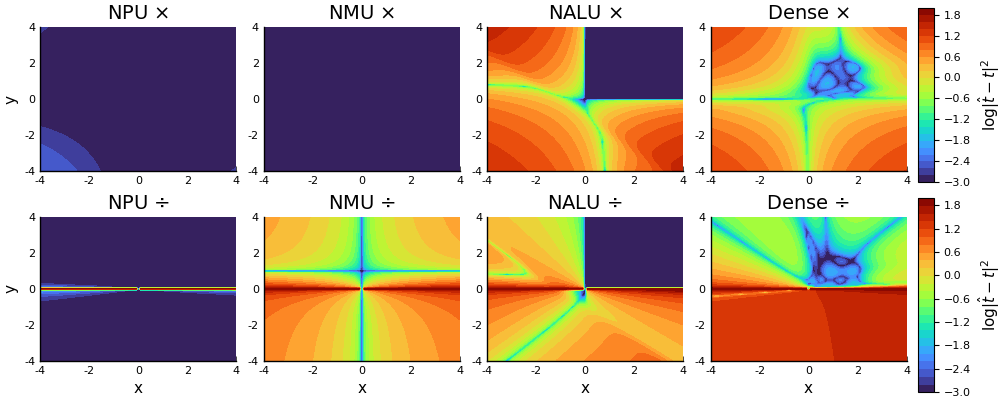
\includegraphics[width=0.8\linewidth]{compare-npu-nmu-nalu-xy-xdivy.png}
  \caption{Comparison of different models learning the function
  $(x,y)\rightarrow(xy,x/y)$ with $(x,y)\in\mathcal U^2(0.1,2)$.  Each
  plot shows the mean-squared error on a logarithmic color scale ($\hat{\bm
  t}=\text{model}(\bm x)$).  The Dense network learns both multiplication and
  division, but fails to extrapolate. NALU learns both tasks perfectly, but
  completely fails if one of the inputs is negative.  The NMU successfully
  learns multiplication, but not division. Only the NPU learns both tasks and
  can extrapolate with an error that is less than $0.01$ in most places.}%
  \label{fig:compare_npu_nmu_nalu_xy_xdivy}
\end{figure}
\todo{add in depth experiment desc. of fig.~\ref{fig:compare_npu_nmu_nalu_xy_xdivy} in appendix}


\section{Neural Power Units}%
\label{sec:neural_power_unit}

Eq.~\ref{eq:nalu_mult} enables the NALU to learn multiplication. If the weight
matrix $\bm W$ would not be restricted to values in the range $(-1,1)$ it could
in principle learn arbitrary power functions, because
\begin{align}
  z = \exp(w\log x) = x^w \text{ for } x>0.
\end{align}

However, this would complicate the convergence issues of the NALU even more.
We therefore suggest to leverage the power of the complex plane, by using the
complex logarithm and by promoting $w$ to a complex number.  This will enable
us not only to lift the positivity constraint on $x$, but also provides and
additional dimension that helps to avoid regions with an uninformative gradient
signal\todo{rephrase this. do we have an educating example where it is obvious
that complex plane helps? the stuff in fig.1 does not work as well with
non-complex NPU, but I have not idea how to plot that}.  Introducing a complex
weight matrix somewhere in a larger network would mean that the gradients in
other layers would potentially become complex as well, which would result in
converting the whole network to complex numbers.  This seems like a high price
to pay, but fortunately there is a way around this.  We can output only the
real part of the result $\real(z)$, but still maintain a complex $w$ by
treating it as a sum of real and imaginary part $w=\wre+i\wim$. We are thus
interested in
\begin{align}
  \label{eq:exp_w_log_complex}
  \real(z) &= \real(\exp(w\log x)),
\end{align}
with a real input $x$. The complex logarithm is defined as $\log z=\log r +
i\theta$, which, for real inputs $x$, can be simplified to $\log z = \log r +
ik\pi$, where $k\in \{0,1\}$. With that Eq.~\ref{eq:exp_w_log_complex} can be
rewritten to
\begin{align}
  \real(z) &= \real(\exp((\wre + i\wim) (\log r + ik\pi))) \\
    &= \exp(\wre\log r - \wim k\pi) \cos(\wim\log r + k\pi\wre),
\end{align}
where we used Euler's formula\footnote{Euler's formula states that for any real
number $x$: $re^{ix} = \cos x + i\sin x$}.
\todo{explicitly compute gradients?}

\subsection{Neural Power Unit (NPU)}%
\label{sub:neural_power_unit_npu_}

\begin{figure}
  \centering
  \resizebox{.3\textwidth}{!}{\input{../plots/exp_log_sin/log_comp.tikz.tex}}
  \resizebox{.3\textwidth}{!}{\input{../plots/exp_log_sin/exp_comp.tikz.tex}}
  \resizebox{.3\textwidth}{!}{\input{../plots/exp_log_sin/sin_comp.tikz.tex}}
  \caption{Function learning comparison of different layers.}%
  \label{fig:sin_comp}
\end{figure}

The \emph{Neural Power Unit} (NPU) with two weight matrices $\Wre$ and $\Wim$
then reads
\begin{align}
  \bm r = |\bm x|,
  \hspace{1cm}
  & k_i = \begin{cases}
     0  & x_i \leq 0 \\
    \pi & x_i > 0
  \end{cases}
\end{align}
\begin{align}
  \bm z &= \exp(\Wre \log\bm r - \Wim\bm k) \odot \cos(\Wim\log \bm r + \Wre\bm k)
\end{align}
where $\bm k$ is a vector that is zero where $\bm x$ is positive and $\pi$
where it is negative, $\bm r$ is the element-wise absolute value.
In the final network we are only interested in real powers, so we recommend to
strongly regularize the imaginary part of the weights $\Wim$.

\subsection{Gated NPU}%
\label{sub:gated_npu}
As pointed out by \cite{madsen_neural_2020}, the loss surface of the NALU, and
thus also the NPU, is not always smooth. For some input and weight combinations
it can happen that the loss close to zero becomes very large as shown in
Fig.~\ref{fig:task_loss_npu_nmu}.
\begin{figure}
  \centering
  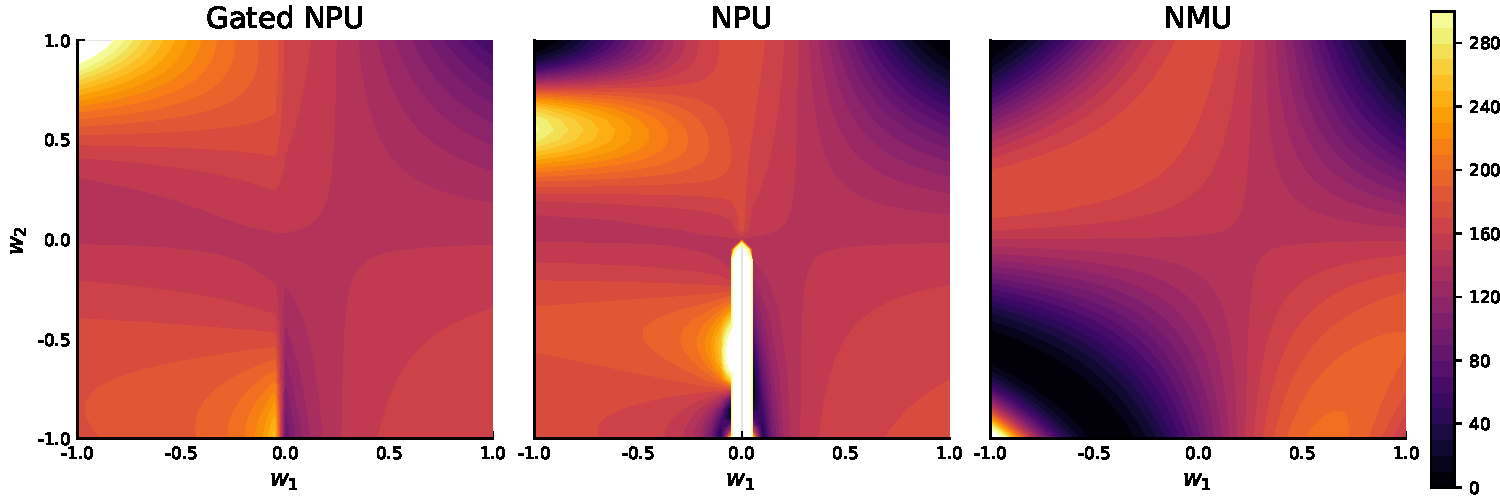
\includegraphics[width=0.8\linewidth]{task_loss_npu_nmu.pdf}
  \caption{asdf}%
  \label{fig:task_loss_npu_nmu}
\end{figure}
However, most applications are dealing with batches of data which average out
these cases, as shown in Fig.~\ref{fig:task_loss_npu_nmu_average} for a batch
size of 32.
\begin{figure}
  \centering
  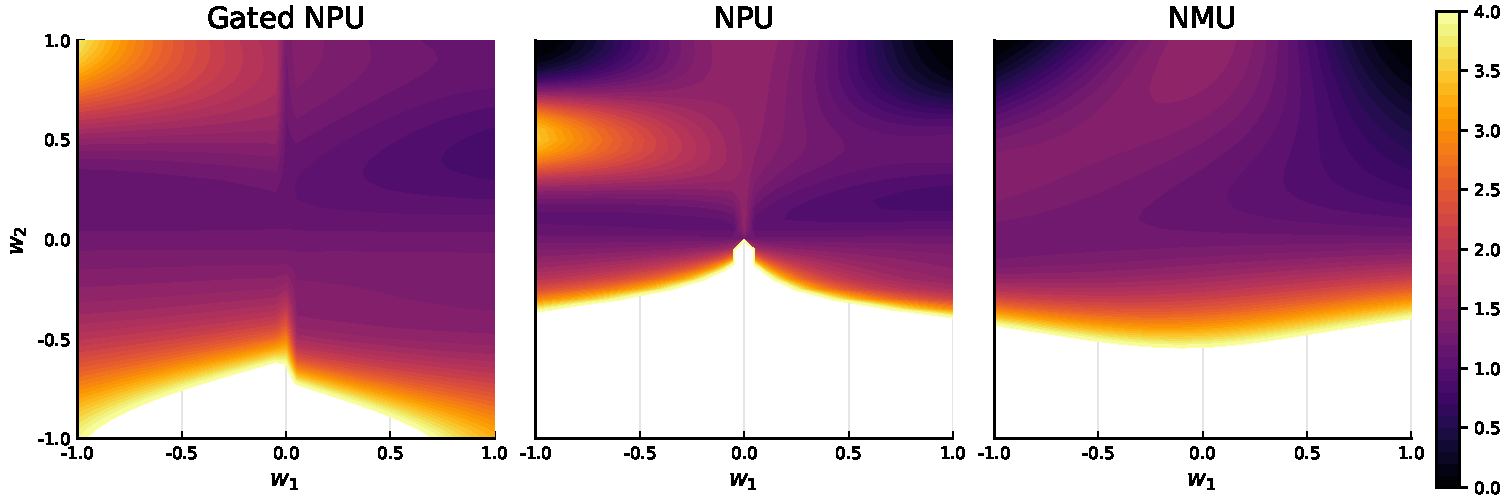
\includegraphics[width=0.8\linewidth]{task_loss_npu_nmu_average.pdf}
  \caption{asdfadsf}%
  \label{fig:task_loss_npu_nmu_average}
\end{figure}

In practice we encountered difficulties of obtaining sparse solutions with the
NPU. If the inputs to an NPU unit are small, the gradient becomes practically
zero, as we can see in Fig.~\ref{fig:id_loss_npu_nmu}
\begin{figure}
  \centering
  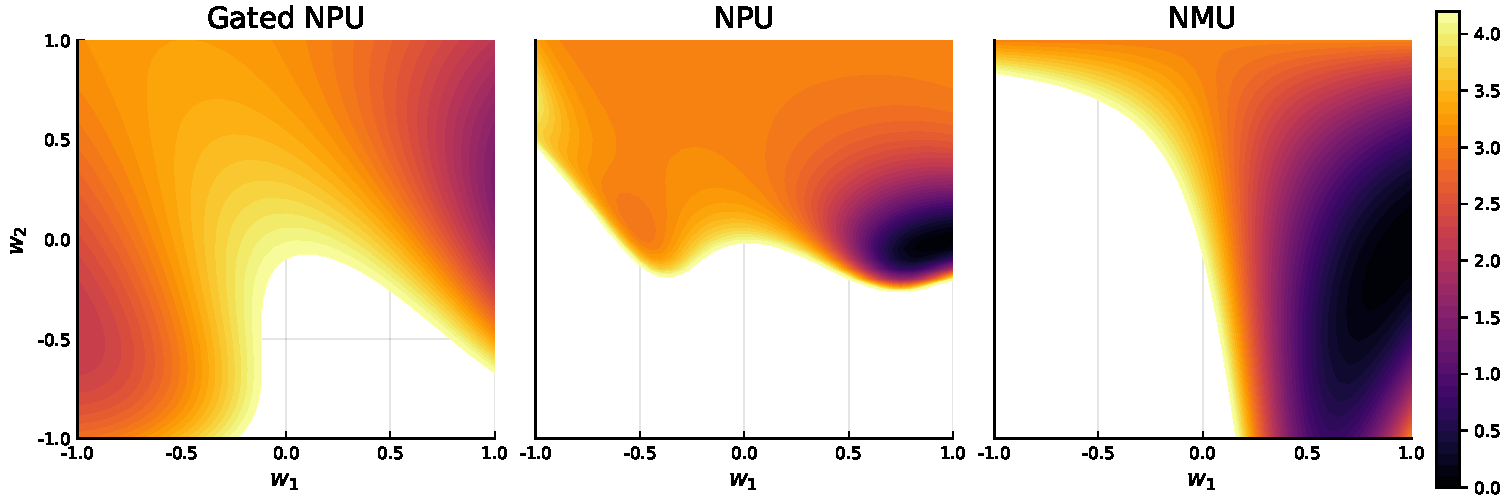
\includegraphics[width=0.8\linewidth]{id_loss_npu_nmu.pdf}
  \caption{learning identity with small inputs}%
  \label{fig:id_loss_npu_nmu}
\end{figure}

\section{Experimetns}%
\label{sec:experimetns}
This can be demonstrated by training a traditional, dense NN to approximate
three functions
\begin{align}
  \label{eq:approx_tasks}
  f(x) = e^x, && g(x) = \log(x), && h(x) = \sin(x)
\end{align}

Neural Arithmetic Units aim to overcome this problem with units that are able
to represent simple arithmetic operations exactly. By composition of these
units it becomes possible to learn e.g. exponentials, logarithms, and power
functions. This promises to improve on the extrapolation capabilities of NNs
even on tasks that are beyond artificial arithmetic tasks such as learning
multiplication, or a certain power function \todo{cite some examples}.


\subsection{10 param func}%
\label{sub:10_param_func}


% \begin{figure}
%   \centering
%   \includegraphics[width=0.8\linewidth]{10-param-func-task-nmu-paper.pdf}
%   \caption{MSE optimization result}%
%   \label{fig:10-param-func-task-nmu-paper}
% \end{figure}
% \begin{figure}
%   \centering
%   \includegraphics[width=0.8\linewidth]{10-param-func-bayes-task-nmu-paper.pdf}
%   \caption{ARD result with MSE starting point}%
%   \label{fig:10-param-func-bayes-task-nmu-paper}
% \end{figure}
% \begin{figure}
%   \centering
%   \includegraphics[width=0.8\linewidth]{10-param-func-bayes-task-nmu-paper-history.pdf}
%   \caption{ARD history}%
%   \label{fig:history}
% \end{figure}
% 
% \subsection{10 param func with sqrt and power}%
% \label{sub:10_param_func_with_sqrt_and_power}
% 
% \begin{figure}
%   \centering
%   \includegraphics[width=0.8\linewidth]{10-param-func-task-sqrt-power.pdf}
%   \caption{10-param-func-task-sqrt-Power}%
%   \label{fig:10-param-func-task-sqrt-power}
% \end{figure}
% \begin{figure}
%   \centering
%   \includegraphics[width=0.8\linewidth]{10-param-func-bayes-task-sqrt-power.pdf}
%   \caption{10-param-func-bayes-task-sqrt-Power}%
%   \label{fig:10-param-func-bayes-task-sqrt-power}
% \end{figure}
% \begin{figure}
%   \centering
%   \includegraphics[width=0.8\linewidth]{10-param-func-bayes-task-sqrt-power-history.pdf}
%   \caption{10-param-func-bayes-task-sqrt-Power-history}%
%   \label{fig:10-param-func-bayes-task-sqrt-power-history}
% \end{figure}


\subsection{Gradient surfaces}%
\label{sub:gradient_surfaces}
% \begin{figure}
%   \centering
%   %\includegraphics[width=0.8\linewidth]{../plots/test.pgf}
%   \input{../plots/test.tikz.tex}
%   \caption{Test}%
%   \label{fig:test}
% \end{figure}

\appendix
\section*{Appendix A}%
\label{sec:appendix_a}

\todo{add sqrt to table~\ref{tab:compare_npu_npu_nalu}?}
\begin{table}[h]
  \centering
  \caption{Comparison of different $2\times2$ layers on the task
  $(x,y)\rightarrow(xy,\frac{x}{y})$.  $(x,y) \in \mathcal U^2(-2,2)$.}
  \label{tab:compare_npu_npu_nalu}
  \begin{tabular}{lcccc}
\toprule
Model & MultTrain & DivTrain & MultTest & DivTest\\
\midrule
NPU & 0.0 & 0.0 & 1.0e-6, & 0.003931 \\
NMU & 0.0 & 2.147657 & 0.0, & 37586.383 \\
NALU & 0.0 & 0.0 & 69.176575, & 140262.12 \\
Dense & 6.7e-5 & 4.7e-5 & 21.469229, & 38017.453 \\
\bottomrule
\end{tabular}

\end{table}



\bibliographystyle{plainnat}
\bibliography{refs}

\end{document}
